
\subsection{Predictions and early evidence for the quark gluon plasma}

Quantum chromodynamics (QCD) describes the interactions of the quarks and gluons (together known as partons) via the strong nuclear force.  The strength of the QCD interactions, described by the QCD coupling constant $\alpha_{s}(Q)$ decreases as distances between strongly interacting partons decreases and their exchanged momentum $Q$: 

\begin{equation}
\label{eq:alpha_s}
\alpha_{s}(Q) \propto \frac{1}{{\rm ln}(\frac{Q^{2}}{\Lambda_{QCD}})}, 
\end{equation}

\noindent where $\Lambda_{QCD} \approx 0.2$ GeV gives the QCD scale.  Figure~\ref{fig:alpha_s} shows the dependence of $\alpha_{s}$ on momentum scale $Q$.  In the regime where separations between partons are relatively large (small $Q$), $\alpha_{s}$ is large, leading to the observed confinement of quarks and gluons in composite particles called hadrons, most commonly baryons (comprised of 3 quarks, including protons and neutrons) and mesons (comprised of 2 quarks).  In the large $Q$ regime, however--accessed via large baryon chemical potential $\mu_{B}$ or large temperature $T$--the strength of the coupling constant $\alpha_{s}$ decreases, in a phenomenon known as asymptotic freedom.  Asymptotic freedom both permits the accurate approximation of high-energy hadron interactions using perturbation theory (pQCD), and implies the deconfinement of quarks and gluons.  This phase of deconfined quarks and gluons, known as the  quark gluon plasma (QGP), was originally conceived as a gas of color-charged quarks and gluons, analogous to the plasma of photons and electrons previously studied in quantum electrodynamics.  In collider studies, this suggests the possibility of a phase transition anticipated between the hadron gas phase present under ordinary matter conditions, and the QGP phase present at sufficiently great $\mu_{B}$ or $T$~\cite{Kalashnikov:1979, Shuryak:1980tp}.

\begin{figure}[h!]
\begin{center}
\includegraphics[width=0.5\textwidth]{figures/Theory/Alpha_s.png}
\caption[QCD coupling constant $\alpha_{s}$]{Momentum scale dependence of QCD coupling constant $\alpha_{s}$, from Ref.~\cite{Bethke:2012jm}.}
\label{fig:alpha_s}
\end{center}
\end{figure}

In the early 1980s, relativistic nuclear collisions were suggested as a means of producing sufficient temperatures and densities to induce a quark-gluon plasma and probe the transition between the QGP and ordinary matter.  Efforts were also made to anticipate key experimental signatures of the short-lived possible QGP, relying in many cases on the anticipation that the QGP would behave according to a hydrodynamic description of a system in at least partial thermal equilibrium.  Proposed signatures included enhancements of strange (heavy) quarks, unusual event structures, greater rates of direct dilepton and photon production~\cite{Bjorken:1983}.  The first heavy ion collisions began with fixed-target experiments at the Super Proton Synchrotron (SPS) at CERN in the mid-1980s, colliding nuclei including gold and lead at energies from 40 GeV to 160 GeV through the 1990s.  Analysis of the hadron yields in these collisions showed an apparent chemical equilibrium of quarks and gluons at about 170 MeV and enhancement (as anticipated) both of strangeness (via kaon/pion ratios, and J/$\psi$ production rates).  In the early 2000, a CERN press release cited these results in declaring that ``a common assessment of the collected data leads us to believe that a new state of matter has indeed been created...[that] features many of the characteristics of the theoretically predicted quark-gluon plasma''~\cite{Heinz:2000bk}.

Shortly after the SPS announcement, the first gold-gold collisions began at the Relativistic Heavy Ion Collider (RHIC) at Brookhaven National Laboratory, beginning an era of high-energy heavy ion collisions that would later be complimented by a parallel program at the Large Hadron Collider at CERN.  Through data collection and analysis by experiments at each of these colliders over the ensuing nearly two decades, the field has gradually shifted from searches for signatures of QGP formation in heavy ion collisions, to detailed characterizations of its properties and evolution.  In 2005, the four experimental collaborations at RHIC (BRAHAMS, PHENIX, PHOBOS, and STAR) published coordinated white papers~\cite{Arsene:2004fa, Adcox:2004mh, Back:2004je, Adams:2005dq} summarizing the assembled evidence that results from  gold-gold collisions could not be explained by models of ordinary hadronic matter--most notably in signatures of collective behavior (see Sec.~\ref{sec:theory_collectivity}) and in suppression of particles with relatively high transverse momentum (see Sec.~\ref{sec:theory_jets}).  Beginning in 2010, heavy ion studies at the LHC by the ALICE, ATLAS, and CMS Collaborations (and more recently by the LHCb Collaboration) have complimented the RHIC access to a wide range of center-of-mass-energies in the 7.7 GeV to 200 GeV range with measurements at 2.76 TeV and 5.02 TeV.

\subsection{Thermodynamics of the quark gluon plasma}

The existence of a plasma phase of hadronic matter and a number of the properties of this phase can also be inferred directly from thermodynamic considerations of hadronic matter.  In free space, the density of states of hadrons as a function of resonance mass $m$ increases exponentionally, following the Hagedorn spectrum

\begin{equation}
\label{eq:hagedorn}
\rho(m) = m^{\frac{5}{2}}e^{\frac{m}{T_{0}}},
\end{equation} 

\noindent where $T_{0} \approx m_{\pi} \approx $ 140 MeV.~\cite{Gyulassy:1985, Sarkar:2010zza}.  When taking into account the finite size of hadrons (with radii on the order of 1 fm), this suggests an upper limit or critical temperature $T_{c} \approx 150$ - 200 MeV above which quark and gluon deconfinement occurs.  The pressure and energy density of this plasma phase are both, to first order in the ideal gas, proportional to $T^4$, with higher order corrections introduced by the non-zero effective (``thermal'') quark and gluon masses.  Defining a color-dependent constant $c$ and a ``bag pressure'' $B$ (named after the MIT model of hadrons as ``bags'' of quarks and gluons) that takes into account the difference between quark and gluon ground states and the vacuum, pressure may be expressed to first order as: 

\begin{equation}
\label{eq:pressure}
P = cT^4 - B,
\end{equation} 

\noindent and energy density $\epsilon$ may be expressed to first order as: 

\begin{equation}
\label{eq:epsilon}
\epsilon = 3cT^4 + B.
\end{equation} 

\noindent Interaction effects due differences between the ground state and the vacuum may be captured by ``interaction measure'' $\Delta = (\epsilon - 3P)/T^{4}$.  Latice QCD studies show a sharp rise in energy density from the low-density hadronic state at the critical temperature $T_{c}$, saturating to constant values at larger $T$.  These values are about 10\% less than those expected for an ideal massless gas due to the higher order thermal mass corrections.  The interaction measure remains non-zero above $T_{c}$, indicative of differences between the vacuum and the QCD ground state or possibly of color resonance states in the QGP.~\cite{Sarkar:2010zza, Satz:2012zza}

Figure~\ref{fig:illustration_qcd_phase_diagram} gives a schematic illustration of the QCD phase diagram as a function of baryon chemical potential and temperature based on thermodynamic considerations and lattice QCD studies.  While chiral symmetry is spontaneously broken for non-zero quark masses, asymptotic freedom implies chiral symmetry at sufficiently large temperatures and a phase transition between the two (hadronic and quark gluon plasma) phases, which is first-order at sufficiently large $\mu_{B}$ with singularities in thermodynamic functions.  Below a certain critical point value of $\mu_{B}$ (and at critical temperature $T_{c}$), however, the transition is a cross-over without singular behavior, and lattice QCD simulations have demonstrated such cross-over behavior for the limit $\mu_{B} = 0$.  This suggests the existence of a tricritical point on the phase boundary between confined and deconfined QCD phases.~\cite{Sarkar:2010zza, Satz:2012zza, Stephanov:2007fk}  The beam energy scan program at RHIC probes center-of-mass energies ranging from 7.2 to 200 GeV to probe temperatures around the predicted values for $T_{c}$;  at LHC energies 2.76 TeV and 5.5 TeV initial QGP temperatures are estimated in the 300 - 700 MeV range, well above the critical temperature.~\cite{Foka2016} 

\begin{figure}[hbtp]
\begin{center}
\includegraphics[width=0.6\textwidth]{illustrations/qcd_phase_diagram.pdf}
\caption[QCD phase diagram]{Schematic phase diagram of strongly interacting matter as a function of baryon chemical potential $\mu_{B}$ and temperature $T$ .}
\label{fig:illustration_qcd_phase_diagram}
\end{center}
\end{figure}

\subsection{Time-evolution of heavy ion collisions}

Connecting predictions and simulations of QGP behavior to experimental results requires the description and analysis of several different sequential phases of heavy ion collisions~\cite{Sarkar:2010zza,Jaiswal:2016hex}:  
\begin{enumerate}
\item \textbf{Initial state} -- Nuclei A and B (lorentz-contracted into two flat discs) approach each other with impact parameter $b$ and nucleon distributions $\rho{A}(r)$ and $\rho{B}(r)$, establishing a set of initial conditions with implications for the later evolution of the medium. 

\item \textbf{Pre-equilibrium} -- Initially after nuclei collide (before thermalization time $\tau_{0}$), nucleons interact dynamically as the QGP begins to form.  Various models -- including IP-Glasma, A Multiphase Transport Model (AMPT), Ultrarelativistic Quantum Molecular Dynamics (UrQMD), and models based on the Anti-deSitter/Conformal Field Theory (ADS/CFT) correspondence -- attempt to capture these dynamics.  

\item \textbf{Hydrodynamic expansion} -- After thermalization time $\tau_{0}$ local thermodynamic equillibrium is achieved, producing an expanding medium whose properties can be described with ideal fluid dynamics with sheer viscocity to energy-density ratio $\eta / s \approx 1.6$ at RHIC and the LHC~\cite{Heinz:2011kt}. 

\item \textbf{Hadronization (``freeze-out'')} -- Quarks and gluons recombine into hadrons in the phase transition back from deconfined to confined QCD matter.  As the medium expands, it reaches sufficiently low densities and temperatures that thermal equilibrium is lost, and quark and gluon recombination stops.  Chemical freeze-out occurs when particle number changing processes end; kinetic freeze-out occurs later, when the ratio of the expansion rate to the collision rate among particles drops to the point that collisions no longer occur.

\item \textbf{Free-streaming} -- recombined hadrons move through the beam pipe vacuum and are measured by the detector.  Experimental results can only directly access these final distributions of particles, from which inferences are made about the other collision stages.  

\end{enumerate}

\noindent Each stage of this QGP time evolution may be accessed via various experimental observables.  Vacuum-like hadronization is well-modeled by parton shower simulations in Monte Carlo generators such as {\sc pythia} and {\sc herwig} that capture proton-proton collision dynamics. Heavy ion collisions, however, present the challenge of defining a freeze-out hypersurface at which hydrodynamic evolution terminates, and hadronization begins. This hypersurface occurs at the phase transition boundary, and may be experimentally accessed via the yields of hadron species in the final state (as particle numbers do not change during the free-streaming stage)~\cite{Sarkar:2010zza}.  Initial collision geometry may be described via Glauber Models and nuclear parton distribution functions (PDFs) of the incoming partons, as discussed in Sec.~\ref{sec:glauber}.  Signatures of initial collision anisotropy and collective hydrodynamic evolution may be observed as ``collective flow'' via particle correlations (Sec.~\ref{sec:theory_collectivity}).  Pre-equilibrium dynamics are particularly difficult to access, but probes including the medium modifications to high-$p_{\rm T}$ jets presented in this analysis provide possiblities for distinguishing between the different theoretical models. 


\subsection{Characterizing collision geometry and event centrality}
\label{sec:glauber}

In heavy ion events there is a wide range of possible collision geometries:  at one extreme the nuclei may colide head-on (refered to as a ``central'' collision, with impact parameter $b=0$), while at the other they may barely graze each other (referred to as a ``peripheral'' collision).  The initial geometry, size, and evolution of the QGP formed in these events may vary considerably based on these initial collisions.  At the most basic level, events may vary in both the number of participating nucleons ($\rm N_{part}$), and in the number of binary nucleon-nucleon collisions ($\rm N_{coll}$) occurring in the event.  While it is not possible to directly measure $b$, $\rm N_{part}$, or $\rm N_{coll}$ in a heavy ion experiment, it is possible to measure the total energy deposited in calorimeters at very forward rapidities along the beam line direction.  The total energy deposited in these forward calorimeters is directly related to the number of ``spectator'' nucleons that do not collide in the event, and therefore inveresely related to to $\rm N_{part}$.  By dividing the total experimental event sample into ``centrality classes'' (ranging from 0\% ``most central'' to 100\% ``most peripheral'') by total energy deposited at forward rapidity and mapping this classification to a simulated sample, it is possible to map events to Monte Carlo simulation and extract mean values for $\rm N_{part}$ and $\rm N_{coll}$~\cite{Miller:2007ri}.

Glauber Models allow for the characterization of event parameters based on modeling of collision geometry.  In the simplest ``optical limit'' of such models, it is assumed that individual nucleons accelearted to very high momenta move relatively independently and linearly, and deflection and shaddowing effects are neglected.  These assumptions reduce the problem to one of only collision geometry, take the inelastic nucleon-nucleon cross-section $\sigma_{NN}^{\rm inel}$ and the density of nucleons in each colliding nucleus $\rho{A}(r)$ and $\rho{B}(r)$ to calculate a ``nuclear overlap function'' $T_{AB}$, defined as: 

\begin{equation}
\label{eq:t_aa}
T_{AB} = \int d^{2}\vec{s} \int dz_{A} \rho{A}(\vec{s}, z_{A}) \int dz_{B} \rho{B}(\vec{s} - \vec{b}, z_{B}),
\end{equation}

\noindent where the integrals  $\int dz_{A} \rho{A}(\vec{s}, z_{A}) $and  $\int dz_{B} \rho{B}(\vec{s} - \vec{b}, z_{B})$ define the probability of finding a nucleon at locations $(\vec{s}, z_{A})$ and $(\vec{s} - \vec{b}, z_{B})$, respectively with the geometry shown in Fig.~\ref{fig:illustration_glauber}.  

\begin{figure}[hbtp]
\begin{center}
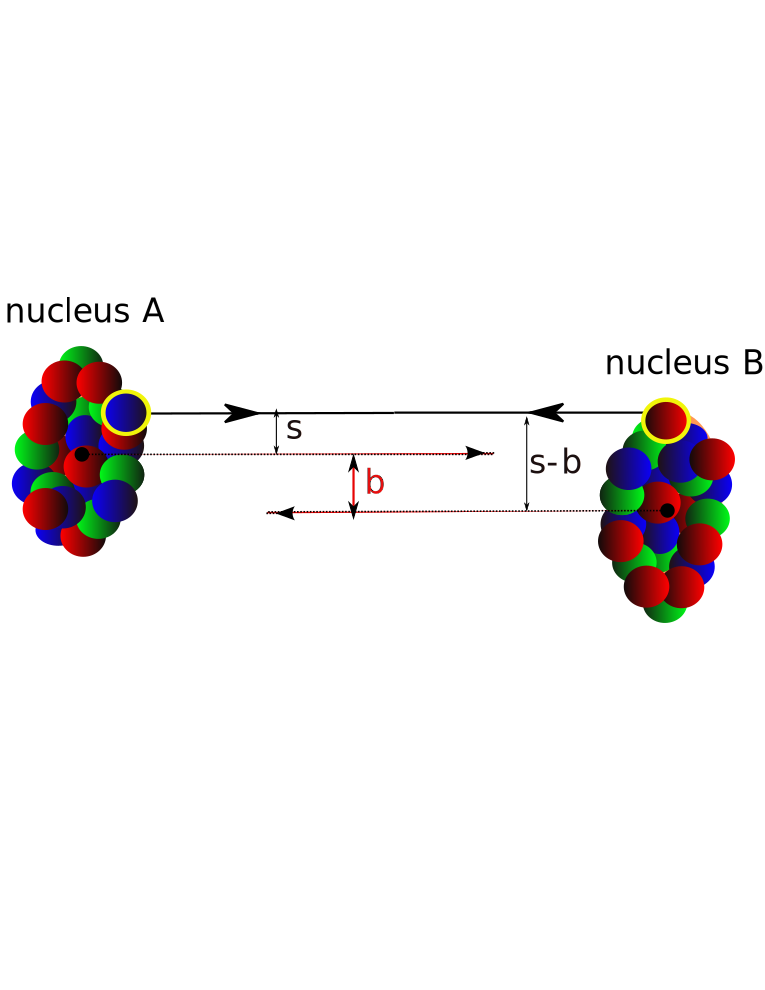
\includegraphics[width=0.6\textwidth]{illustrations/glauber.pdf}
\caption[Glauber model illustration]{Schematic illustration of Glauber Model geometry for a nucleus-nucleus collision, showing impact parameter $\vec{b}$ between the two nuclei and locations of two representative colliding nuclei.}
\label{fig:illustration_glauber}
\end{center}
\end{figure}

\noindent The resulting total number of collisions is then given by: 

\begin{equation}
\label{eq:n_coll}
{\rm N_{coll}}(b) = \sigma_{NN}^{\rm inel} T_{AB}(b).
\end{equation}

\noindent For example for minimum bias collisions at LHC energy 2.76 TeV $\sigma_{NN} = 65$ mb, $\sigma_{\rm PbPb} = 7660$ mb, $\langle T_{\rm PbPb} \rangle = \int d^2 b T_{\rm PbPb} / \int d^2 b = 5.65 {\rm mb}^{-1}$, and $\langle {\rm N_{coll}}(b) \rangle = 367$~\cite{Miller:2007ri, dEnterria:2003xac}.  The optical limit calculations described above are able to reasonably capture collision parameters, but are limited by their neglect of effects including nuclear shadowing and diffraction.  Glauber Monte Carlo simulations are able to re-introduce some of these effects, thereby better capturing the nuclear cross section~\cite{Miller:2007ri, Majumder:2010qh}.  

\subsection{Kinematic variables and coordinates}

In high-energy colliders the $z$ axis is defined parallel to the colliding beams, with $x$ and $y$ axes spanning a transverse plane perpendicular to the beam axis.  Because the colliding nuclei are accelerated to nearly the speed of light, it is necessary to use relativistic coordinates starting from the energy-momentum relationship:

\begin{equation}
\label{eq:energy_momentum}
E^{2} = p_{x}^{2}c^{2}+p_{y}^{2}c^{2}+p_{z}^{2}c^{2}+M^{2}c^{4}
\end{equation}

\noindent for a particle with rest mass $M$.  The azimuthal coordinate in the transverse plane is then simply given by: 

\begin{equation}
\label{eq:phi}
\phi = {\rm tan}^{-1}\Big(\frac{p_{y}}{p_{x}}\Big)
\end{equation}

\noindent With incoming particles colliding with very large $p_{z}$, the outgoing direction of collision products is characterized by their rapidity $y$, a generalization of velocity defined by: 

\begin{equation}
\label{eq:rapidity}
y = {\rm ln} \sqrt{\frac{E+p_{z}c}{E-p_{z}}},
\end{equation}

\noindent The rapidity is defined such that particles which emerge perpendicular to the beam axis (with $p_{z}=0$) have $y = 0$, while $y \rightarrow \infty$ toward the beam line.  In practice, however, the outgoing particle's rest mass $M$ and energy $E$ are generally unknown, while the total momentum $\vec{p}$ can be measured in detectors.  In ultrarelativistic collisions, where $\vec{p}^{2} > > M^2c^2$, we instead measure the pseudorapdity $\eta$ defined by: 

\begin{equation}
\label{eq:eta}
\eta = {\rm ln} \Big(\frac{|\vec{p}|+p_{z}}{|\vec{p}|-p_{z}}\Big)
\end{equation}

\noindent Pseudorapidity may also be calculated from the polar angle $\theta$ with respect to the beam pipe,

\begin{equation}
\label{eq:eta2}
\eta = \rm{-ln\Big(tan\Big(\frac{\theta}{2}\Big)\Big)}
\end{equation}

\noindent As is clear from this representation, particles perpendicular to the beampipe with $\theta = \pi/2$ correspond to rapidity $\eta = 0$, while particles with $\theta = \pi/4$ correspond to $\eta \approx 0.88$.  

In general throughout this document, energies and measurements are presented in natural units with $\hbar = c = 1$ (momenta, for example, are given in MeV or GeV rather than MeV/c or GeV/c).  Azimuthal angle $\phi$ is measured in radians.  

\subsection{Collective behavior in the QGP}
\label{sec:theory_collectivity}

In any nucleus-nucleus collision, the initial collision region will exhibit some azimuthal anisotropy--both due to the elliptical overlap region for collisions with impact parameter $b > 0$, and due to local variations in the nuclear densities $\rho{A}$ and $\rho{B}$.  As the medium thermalizes and hydrodynamically expands, this spatial anisotropy translates into anisotropy in momentum space or ``collective flow'' of the expanding medium.  This correlation is retained through the hadronization and free-streaming phases, and is ultimately detectable via modulation in the distribution of particles with respect to the reaction plane ($\psi_{RP}$, the plane spanned by the impact parameter $\vec{b}$ and the beam direction).  This may be expanded in a Fourier series, 

\begin{equation}
\label{eq:collective_flow_rp}
\frac{dN}{d\phi} = \frac{N}{2\pi} \Big(1+2\Sigma_{n} v_{n} {\rm cos}(n(\phi - \psi_{RP}))\Big),
\end{equation}

\noindent using Fourier coefficients $v_{\rm 1}$, $v_{2}$, $v_{3}$, etc. (sometimes referred to as ``harmonic flow coefficients'') to model the $\Delta\phi$ correlation between particles and the reaction plane.  These coefficients may be interepreted as corresponding to different geometric anisotropies in the initial state:  $v_{1}$ refers to  ``directed flow'' which arises as colliding nucleons are repelled perpendicular to the beam direction int he reaction plan.  Elliptic flow coefficient $v_{2}$ refers to the elliptical anisotropy arising from the overlap of two roughly circular nuclei, while $v_{3}$ (``triangular flow'') and higher coefficients refer to more complex initial geometries arising from fluctuations in the nucleon densities~\cite{Voloshin:2008dg}.

The azimuthal direction of the reaction plane $\psi_{RP}$ cannot be directly experimentally measured, but may be estimated based on event-by-event particle distributions in the detector.  Alternatively, flow may be measured by considering two-particle correlations measuring $\Delta\phi_{\rm trig, assoc}$ between trigger and associated particles.   In this case, the Fourier decomposition of the $\Delta\phi_{\rm trig, assoc}$ distribution becomes


\begin{equation}
\label{eq:collective_flow_dihad}
\frac{1}{N_{\rm trig}} \frac{dN^{\rm pair}}{d\Delta\phi_{\rm trig, assoc}} = \frac{N_{\rm assoc}}{2\pi} \Big(1+2\Sigma_{n} V_{n} {\rm Cos}(n(\Delta\phi_{\rm trig, assoc}))\Big),
\end{equation}

\noindent Here the combined flow coefficients $V_{n}$ are found to be factorizable into coefficients for the trigger and associated hadrons, i.e. $V_{n} = v_{n, {\rm trig}} \times v_{n, {\rm assoc}}$~\cite{Chatrchyan:2011eka, Chatrchyan:2013nka}.  To measure collective flow through this two-particle method, two dimensional correlations in $\Delta\eta-\Delta\phi$ are constructed between trigger and associated hadrons, as shown in Fig.~\ref{fig:cms_dihadron_2D} from CMS study~\cite{Chatrchyan:2013nka}.  These distributions are projected over the large $\Delta\eta$ region (in this case $|\Delta\eta| < 2$ to capture long range correlations, and are fit in $\Delta\phi$ with the Fourier function shown above to extract flow coefficients $V_{1}$, $V_{2}$, and $V_{3}$, from which $v_{1}$, $v_{2}$, and $v_{3}$ may be calculated.  These studies find centrality- and $p_{\rm T}$-dependent flow coefficients through $v_{3}$, with $v_{3}$ present substantially smaller than $v_{2}$.  As expected from simple geometrical considerations, values of $v_{2}$ and $v_{3}$ are greatest for mid-central collisions in which collision anisotropy is greatest, and peak as a function of $p_{\rm T}$ in the 2-3 GeV range, as shown in Fig.~\ref{fig:cms_v2_v3_result}.  

\begin{figure}[hbtp]
\begin{center}
\includegraphics[width=0.5\textwidth]{figures/Theory/CMS_2particle_corr_2D.pdf}
\caption[Dihadron correlation in $\Delta\eta-\Delta\phi$]{Illustraiton of dihadron correlation in $\Delta\eta-\Delta\phi$ for $1< p_{\rm T}^{\rm trig} < 3$ GeV and $1< p_{\rm T}^{\rm assoc} < 3$ GeV in central PbPb collisions at 2.76 TeV from Ref.~\cite{Chatrchyan:2013nka}}
\label{fig:cms_dihadron_2D}
\end{center}
\end{figure}

\begin{figure}[hbtp]
\begin{center}
\includegraphics[width=0.99\textwidth]{figures/Theory/CMS_2particle_corr_fits.pdf}
\caption[Fits to dihadron $\Delta\phi$ distributions to extract flow coefficients]{Fourier fits to dihadron $\Delta\phi$ distributions for  $1< p_{\rm T}^{\rm assoc} < 2$ GeV as a function of $p_{\rm T}^{\rm trig}$ in central PbPb collisions at 2.76 TeV from Ref.~\cite{Chatrchyan:2013nka}}
\label{fig:cms_dihadron_fits}
\end{center}
\end{figure}

\begin{figure}[hbtp]
\begin{center}
\includegraphics[width=0.99\textwidth]{figures/Theory/CMS_v2_v3_result.pdf}
\caption[Flow coefficients $v_{2}$ and $v_{3}$ by centrality and $p_{\rm T}$]{Flow coefficients $v_{2}$ and $v_{3}$ by centrality and $p_{\rm T}$ at 2.76 TeV from Ref.~\cite{Chatrchyan:2013nka}}
\label{fig:cms_v2_v3_result}
\end{center}
\end{figure}


\clearpage

\section{Jets as probes of the quark gluon plasma}
\label{sec:theory_jets}

Hard scatterings in heavy ion collisions can provide powerful probes of the quark gluon plasma.  Because of asymptotic freedom, high-energy parton-parton processes can be accurately characterized via pQCD, and have been thoroughly studied experimentally in hadron-hadron collisions.  In heavy ion collisions, the initial parton-parton interaction should by causality behave the same as a parton-parton interaction in hadron-hadron collisions.  After the collision, however, outgoing partons traverse the quark gluon plasma, providing the opportunity to study medium properties by comparing heavy ion results to expectations inferred from hadron-hadron ``vacuum'' reference data.  These studies are facilitated by the ``factorization theorem'' in pQCD, which states that the cross section $\sigma_{AB\rightarrow h}^{\rm hard}$ of hadron $h$  produced in the hard process $ A + B \rightarrow h$) can be decomposed into contributions from:  

\begin{itemize}
\item The perturbative cross section of the parton hard scattering $\sigma_{ab\rightarrow c}^{\rm hard}$ 
\item The initial parton distribution functions (PDFs) of partons in the colliding nuclei A and B ($f_{a/A}$ and $f_{b/B}$ for partons of flavor $a$ and $b$)
\item The fragmentation function $\mathscr{D}_{c\rightarrow h}$ describing the probability that parton $c$ fragments into hadron h with momentum fraction $z = p_{h}/p_{c}$ 
\end{itemize}

\noindent The total cross section may be represented, schematically, as:  

\begin{equation}
\label{eq:factorization}
d \sigma_{AB\rightarrow h}^{\rm hard} = f_{a/A}(x_{a},Q^{2})  f_{b/B}(x_{b},Q^{2}) \times d \sigma_{ab\rightarrow c}^{\rm hard}(x_{a},x_{b},Q^{2}) \times \mathscr{D}_{c\rightarrow h}(z,Q^{2}),
\end{equation}

\noindent Each contribution to $d \sigma_{AB\rightarrow h}$ can be experimentally determined, and in hadron-hadron collisions $\sigma_{ab\rightarrow c}^{\rm hard}$, fragmentation functions, and PDFs should each be universal.  Figure~\ref{fig:illustration_qgp_factor} illustrates this factorization for hard-scattering interaction $A+B \rightarrow h$.  The final state parton branching is given by the Dokshitzer-Gribov-Lipatov-Altarelli-Parisi (DGLAP) equations that encode the QCD radiation probabilities for a parton propagating in the vacuum.  

\begin{figure}[hbtp]
\begin{center}
\includegraphics[width=0.4\textwidth]{illustrations/qcd_factor.pdf}
\caption[Illustration of QCD cross section factorization]{Illustration of the QCD hard-scattering $A+B \rightarrow h$.}
\label{fig:illustration_qgp_factor}
\end{center}
\end{figure}

The partonic cross section $\sigma_{ab\rightarrow c}^{\rm hard}$ furthermore should not, by causality, depend on the presence or absence of the QGP.  Medium modifications may enter at two phases in this process:  first, via energy loss by parton $c$ passing through the medium, and second via possible medium-induced changes to fragmentation functions $\mathscr{D}_{c\rightarrow h}$.  Parton energy loss is attributed to two primary mechanisms:  collisional energy loss from scatterings with partons in the medium, and medium induced radiation roughly analogous to electromagnetic ionization in a medium~\cite{Bjorken:1982tu, d'Enterria:2009am}.  This medium-induced parton energy loss implies an observable reduction of medium properties can also be further probed by comparing measurements of jet substructure in heavy ion collisions compared to pp reference data (Sec.~\ref{sec:jff_jetshapes}), and by studying modifications to $p_{\rm T}$ balance in back-to-back dijet events (Sec.~\ref{sec:dijet_balance}).

\subsection{Measuring suppression of high-$p_{\rm T}$ particles and jets}
\label{sec:raa}

One observable to probe parton energy loss in the medium is to compare yields of both particles with relatively high transverse momentum ($p_{\rm T}$), and of reconstructed jets (collections of particles clustered in an effort to reconstruct the original parton energy -- see Sec.~\ref{sec:Jets}).  This reduction in jet yields compared to expectations from ``vacuum'' reference or scaled binary collisions can be studied as both a signature of the presence of the QGP, and an observable to distinguish between models of interactions within the QGP (see Sec.~\ref{sec:raa}).  

Since by pQCD factorization the partonic cross-section $\sigma_{ab\rightarrow c}$ should be independent, in the absence of the quark gluon plasma, the nuclear inclusive cross section would be expected to scale with the number of participating nucleons, i.e.  

\begin{equation}
\label{eq:raa_p0}
d \sigma_{AB\rightarrow h}^{\rm hard}(b) = \langle T_{AB}(b) \rangle \sigma_{\rm pp}^{\rm hard}
\end{equation}

\noindent where $T_{AB}(b)$ parameterizes the probability of nucleon-nucleon interactions for a given impact parameter for nucleii A and B colliding with impact parameter $b$ as discussed in Sec.~\ref{sec:glauber}.  A comparison of actual hadron (or jet) yields compared to this expectation can therefore give information about parton interactions with the medium, as characterized by the nuclear modification factor $R_{AA}$ defined as the ratio of the observed yield in heavy ion data to the expecation from binary scaled pp data: 

\begin{equation}
\label{eq:raa_trk}
R_{AA}(p_{\rm T}, \eta) = \frac{d^{2}\sigma_{AA}/dp_{\rm T} d\eta}{\langle T_{AB}(b) \rangle  d^{2}\sigma_{\rm pp}/dp_{\rm T} d\eta}
\end{equation}

Consistent with quenching expectations, RHIC measurements of $R_{AA}$ in gold-gold collisions showed substantial suppression of a factor of 70-80\% for $p_{\rm T} > 4$ GeV~\cite{Arsene:2004fa, Adcox:2004mh, Back:2004je, Adams:2005dq}.  Comparisons of RHIC measurements to early LHC results showed similar qualitative features, but greater suppression at low-$p_{\rm T}$ at the LHC, despite the more slowly falling pp spectrum at the LHC, as shown in Fig.~\ref{fig:alice_chpart_raa}.  Measurements at the LHC have also found that $R_{AA}$ rises with $p_{\rm T}$ for charged particles with $p_{\rm T} > 7$ GeV, and have shown no significant center-of-mass energy differences when comparing $R_{AA}$ at 2.76 TeV and 5.02 TeV, as shown in Fig.~\ref{fig:cms_chpart_raa}.  The $p_{\rm T}$ dependence of $R_{AA}$ is generally driven by three factors:  the kinematic constraints on jet energy loss (model-specific details will be discussed in Sec.~\ref{sec:theory_models}), the fact that $R_{AA}$ takes the ratio of two steeply falling spectra the scattered partons, one shifted by energy loss and one un-shifted, and the effects of nuclear shadowing and anti-shadowing in the nuclear PDFs~\cite{d'Enterria:2009am, Armesto:2006ph}.

\begin{figure}[h!]
\begin{center}
\includegraphics[width=0.5\textwidth]{figures/Theory/ChPart_Raa_ALICE_RHIC.pdf}
\caption[Charged particle $R_{AA}$ at 200 GeV and 2.76 TeV]{Measurements of charged particle $R_{AA}$ from the STAR and PHENIX Collaborations at 200 GeV at RHIC, compared to ALICE results from the LHC at 2.76 TeV from Ref.~\cite{Aamodt:2010jd}.}
\label{fig:alice_chpart_raa}
\end{center}
\end{figure}

\begin{figure}[ht!]
\begin{center}
\includegraphics[width=0.5\textwidth]{figures/Theory/ChPart_Raa_CMS_LHC.pdf}
\caption[Charged particle $R_{AA}$ at 2.76 and 5.02 TeV]{Measurements of charged particle $R_{AA}$ at LHC energies 2.76 TeV and 5.02 TeV from Ref.~\cite{Khachatryan:2016odn}.}
\label{fig:cms_chpart_raa}
\end{center}
\end{figure}


Studies of high-$p_{\rm T}$ tracks make use of the fact that such tracks are likely to originate from outgoing partons in hard-scattering interactions, providing an indirect look at energy loss by the parton used as a probe of the QGP.  To more directly reconstruct parton energy, we may instead consider reconstructed jets, defined as the collection of (spatially grouped) particles resulting from the fragmentation of a high-$p{\rm T}$ quark or gluon.  Jet reconstruction, described in detail in Sec.~\ref{sec:Jets}, groups detector deposits to reconstruct a jet energy, and uses Monte Carlo simulation to reconstruct a ``true'' jet energy of the original parton.  Quenching studies with reconstructed jets therefore can offer a more direct look at energy loss in the medium by comparing measured energy in jets in heavy ion collisions to those in proton-proton collisions.  Measurements of jet $R_{AA}$ at the LHC reported in Refs.~\cite{Aad:2014bxa, Khachatryan:2016jfl} show suppression by a factor of approximately 40-60\% in most central PbPb collisions, with weak depenence on jet $p_{\rm T}$ as shown in Fig.~\ref{fig:cms_jet_raa}.  

\begin{figure}[h!]
\begin{center}
\includegraphics[width=0.99\textwidth]{figures/Theory/JetRaa_CMS.png}
\caption[Jet $R_{AA}$ at 2.76 TeV]{Jet $R_{AA}$ at 2.76 TeV from Ref.~\cite{Khachatryan:2016jfl}.}
\label{fig:cms_jet_raa}
\end{center}
\end{figure}


Jet $R_{AA}$ measurements capture parton energy loss by measuring the reduction in yields in the presence of the QGP.  To connect jet $R_{AA}$ to charged particle $R_{AA}$ measurements, it is necessary to also consider trends in jet fragmentation patterns with jet-$p_{\rm T}$.  High-$p_{\rm T}$ jets are more likely to originate from quarks than from gluons, and therefore exhibit ``harder'' fragmentation patterns--i.e. higher-$p_{\rm T}$ jets fragment into relatively fewer particles each with more $p_{\rm T}$ compared to jets at lower-$p_{\rm T}$.  Jets with softer fragmentation are also expected to exhibit greater modification in the QGP, as low-$p_{\rm T}$ fragmentation products rescatter in the medium.  The highest-$p_{\rm T}$ tracks, for which $R_{AA}$ is the smallest, are associated with those jets that have not only the highest-$p_{\rm T}$, but also the hardest fragmentation.  The high-$p_{\rm T}$ sector of jet $R_{AA}$ measurements at LHC energies, however, still includes significant contributions from jets reconstructed from softer particles that exhibit significant suppression.

\clearpage

\subsection{Jet fragmentation function and jet shape measurements}
\label{sec:jff_jetshapes}

Measurements of jet $R_{AA}$ quantify the overall reduction in numbers of high-$p_{\rm T}$ jets passing a certain momentum threshold, providing an indication of the magnitude of jet energy loss in different $p_{\rm T}$ regions.  As discussed above, this measurement can constrain the possible mechanisms of jet energy loss.  To further constrain models of jet energy loss, additional observables aim to capture the details of jet fragmentation and its modification in the quark gluon plasma.  One such measurement is the jet fragmentation function, which captures the $p_{\rm T}$ distribution of tracks carying jet momentum, paramaterized via the variables $z$ and $\zeta$: 

\begin{equation}
\label{eq:jff_cms}
z = \frac{p^{\rm track}_{\rm ||}}{p^{\rm jet}_{\rm ||}}, \zeta = \frac{1}{{\rm ln} (z)},
\end{equation}

\noindent where $p^{\rm track}_{\rm ||}$ refers to the component of the track $p_{\rm T}$ along the jet axis.  Jet fragmentation function measurements from CMS shown in Fig.~\ref{fig:cms_jff} show a centrality-dependent modification to fragmentation function in PbPb relative to pp data, with a depletion in the mid-$\zeta$ range, balanced by an enhancement at large $\zeta$, in the region corresponding to low-$p_{\rm T}$ tracks.  This shows a redistribution of energy within the jet cone toward softer particle production in the presence of the medium, consistent with predictions of parton energy loss corresponding to a suppression of high-$p_{\rm T}$ particles (model details will be discussed in Sec.~\ref{sec:theory_models}).

\begin{figure}[h!]
\begin{center}
\includegraphics[width=0.99\textwidth]{figures/Theory/CMS_JFF.png}
\caption[Jet fragmentation function in 2.76 TeV PbPb and pp data]{Jet fragmentation function for jets with $100 < p_{\rm T} < 300$ GeV in 2.76 TeV PbPb and pp data from Ref.~\cite{CMS:2012vba}.}
\label{fig:cms_jff}
\end{center}
\end{figure}

In addition to characterizing the $p_{\rm T}$ spectrum of jet constituents, the distribution of $p_{\rm T}$ with respect to the jet axis can also help to constrain fragmentation scenarios.  This distribution, known as the jet shape, is defined within the jet cone as: 

\begin{equation}
\label{eq:jet_shape_cms}
\rho(\Delta r) = \frac{1}{\delta r}\frac{1}{N^{\rm jet}} \mathlarger{ \sum \limits_{\rm jets}} \frac{\Sigma_{{\rm tracks}\in[r_{a},r_{b})} p_{\rm T}^{\rm track}}{p_{\rm T}^{\rm jet}},
\end{equation}

\noindent where $r_{a}$ and $r_{b}$ correspond to the inner and outer radii, respectively, of an annulus of width $\delta r = 0.5$ around the jet axis.  The first jet shape measurement from CMS, shown in Fig.~\ref{fig:cms_jet_shape} (measured with particles with $p_{\rm T} > 1$ GeV), shows a spatial redistribution of energy from small radii ($\Delta r \approx 0.1$) to larger radii ($\Delta r > 0.2$) from the jet axis.  This is qualitatively consistent with predictions of energy redistribution into particles that are both relatively soft ($p_{\rm T} < 3 $ GeV, as observed in jet fragmentation function measurements), and recovered at relatively large angles from the jet axis.  In this way, the study of jet shape modifications $within$ the jet cone motivate extension of these measurements to larger angles from the jet axis to quantify the distribution and $p_{\rm T}$ composition of particles at angles larger than $\Delta r = 0.3$.  

\begin{figure}[hbtp]
\begin{center}
\includegraphics[width=0.99\textwidth]{figures/Theory/CMS_JetShapes.png}
\caption[Jet shape measurement in 2.76 TeV PbPb and pp data]{Jet shape measurement in 2.76 TeV PbPb and pp data from Ref.~\cite{Chatrchyan:2013kwa}.}
\label{fig:cms_jet_shape}
\end{center}
\end{figure}


\clearpage 

\subsection{Dijet asymmetry and momentum balance studies}
\label{sec:dijet_balance}

Additional possibilities for exploration of medium properties follow from the consideration of ``dijets,'' jets that are back-to-back in azimuthal angle ($\Delta \phi_{\rm jets} \approx \pi$).  As the incoming collision participants each begin with $p_{\rm T} \approx 0$ GeV, the total $p_{\rm T}$ of outgoing partons immediately after the collision must also be 0.  If both partons experience either no energy loss (as in the vacuum) or approximately equal energy loss (i.e. by experiencing roughly equal path-lengths through the medium), the measured $p_{\rm T}$ of each jet in the dijet pair would be approximately equal.  If, however, the hard-scattering occurs toward the surface of the QGP, the jet with a longer path-length through the medium might be expected to experience substantially more energy loss, leading to a $p_{\rm T}$ asymmetry in the dijet pair as illustrated in Fig.~\ref{fig:illustration_dijets}.  This expectation was probed via studies of di-hadron correlations with high-$p_{\rm T}$ particle triggers ($4 < p_{\rm T} < 6$ GeV by STAR at RHIC, $8 < p_{\rm T} < 15 $ GeV by ALICE at the LHC) showed results consistent with the expectation.  These studies showed the substantial suppression (even disappearance, in the STAR studies) of yields of particles with $p_{\rm T} > 2$ GeV in the region opposite the trigger hadron in azimuth~\cite{Adler:2002tq, Aamodt:2011vg}, consistent with path-length dependent jet quenching and a surface bias in trigger particles.  

\begin{figure}[hbtp]
\begin{center}
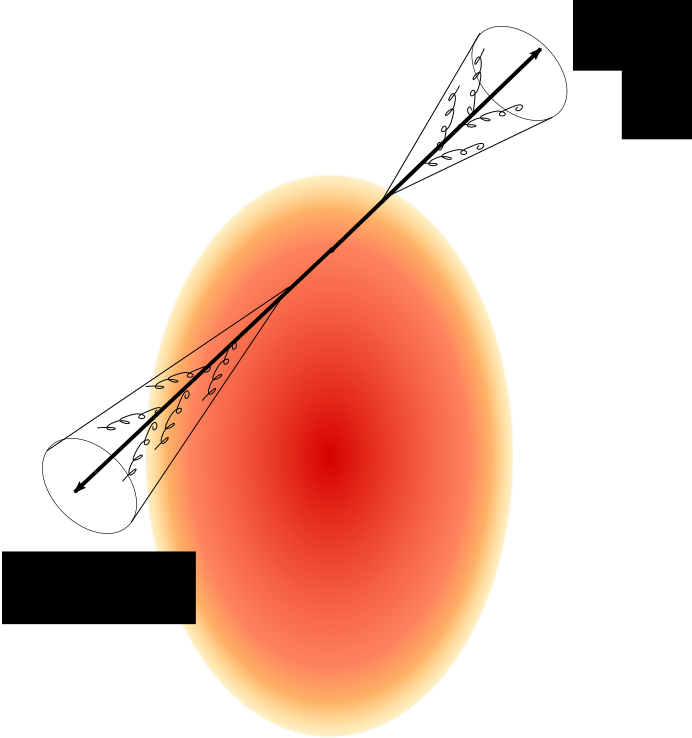
\includegraphics[width=0.3\textwidth]{illustrations/asymmetric_dijets.pdf}
\caption[Illustration of dijet asymmetry]{A ``back-to-back'' pair of dijets separated by $\Delta\phi = \pi$, with a highest-$p_{\rm T}$ leading jet experiencing less quenching in the medium, and a more-quenched subleading jet with a longer path length through the medium.}
\label{fig:illustration_dijets}
\end{center}
\end{figure}


The large kinematic reach of hard probes at the LHC allows for dijet studies at much higher $p_{\rm T}$.  The first of these studies measured the ``dijet imbalance'' between the highest-$p_{\rm T}$ (``leading jet,'' with $p_{\rm T,1}$) and second-highest-$p_{\rm T}$ jets (``subleading jet,'' with $p_{\rm T, 2}$ in the event, parameterized as: 

\begin{equation}
\label{eq:aj}
A_{\rm J} = \frac{p_{\rm T,1} - p_{\rm T,2}}{p_{\rm T,1} + p_{\rm T,2}}
\end{equation}

\noindent These studies, by the ATLAS and CMS Collaborations~\cite{Aad:2010bu, Chatrchyan:2011sx} showed a centrality-dependent shift in the $A_{\rm J}$ in PbPb collisions, with greater dijet asymmetry in central PbPb data than in pp or in peripheral PbPb collisions.  In pp and peripheral PbPb collisions, asymmetric dijet events are those in which some $p_{\rm T}$ is carried by a third jet, and the $A_{\rm J}$ distribution is steeply falling.  In central PbPb collisions, however, there are expected to be two contributions to the sameple of asymmetric dijet events: not only three-jet events, but also dijet events in which the subleading jet is substantially quenched.  As shown Fig.~\ref{fig:cms_dijets}, this effect is evident in the shift toward larger values of $A_{\rm J}$ in central PbPb collisions. 

\begin{figure}[hbtp]
\begin{center}
\includegraphics[width=0.9\textwidth]{figures/Theory/CMS_dijets.png}
\caption[Dijet asymmetry and in 2.76 TeV PbPb and pp data]{Dijet asymmetry in 2.76 TeV PbPb and pp data for jet selection $p_{\rm T,1} > 120$ GeV, $p_{\rm T,2} > 50$ GeV, and $\Delta\phi_{\rm 1,2} > 2\pi/3$ from Ref.~\cite{Chatrchyan:2011sx}.}
\label{fig:cms_dijets}
\end{center}
\end{figure}

The transverse momentum difference between the leading and subleading jets may be conceptualized as ``missing-$p_{\rm T}$'' from the subleading jet, which must by momentum conservation be recovered somewhere in the hemisphere of the event surrounding the subleading jet axis.  One way to capture this momentum balance is by comparing the total $p_{\rm T}$ carried by tracks in different $p_{\rm T}$ classes in the subleading relative to the leading hemisphere.  This balance is shown in the top row Fig.~\ref{fig:cms_mpT}, for $\slashed{p}_{\rm T}^{\rm ||}$ defined as the projection of each track's $p_{\rm T}$ projected in $\phi$ onto the dijet axis (i.e. the average of the leading and subleading jet axes)~\cite{HIN_2014_010}.  In pp and peripheral PbPb data, this balance shows the depletion of tracks with $p_{\rm T} > 8$ GeV in the subleading relative to the leading hemisphere balanced primarily by tracks with $2 < p_{\rm T} < 8$ GeV, consistent with the localization of these tracks in additional jets for unbalanced dijets in this scenario.  The magnitude of the ``missing-$p_{\rm T}$'' balancing distribution increases with growing $A_{\rm J}$ by construction.  Comparing PbPb to pp distributions (differences shown int he bottom row of Fig.~\ref{fig:cms_mpT}), the balancing distribution in unbalanced (large $A_{\rm J}$) events in central PbPb data shows larger contributions from soft particles with $p_{\rm T} < 2$ GeV and smaller contributions from particles with $p_{\rm T} > 4$ GeV, indicating that the more of the balancing $p_{\rm T}$ distribution in the subleading side is carried by soft quenching products rather than additional jets. 


\begin{figure}[hbtp]
\begin{center}
\includegraphics[width=0.99\textwidth]{figures/Theory/CMS_mpT.pdf}
\caption[Hemisphere momentum balance in dijet events as a function of $A_{\rm J}$]{Top row: hemisphere $p_{\rm T}$ momentum balance in dijet events as a function of $A_{\rm J}$, taking the total difference $\slashed{p}_{\rm T}^{\rm ||}$ in the subleading hemisphere minus that in the leading hemisphere from Ref.~\cite{HIN_2014_010} in pp and PbPb data.  Bottom row:  Differences PbPb - pp.}
\label{fig:cms_mpT}
\end{center}
\end{figure}

Dijet momentum balance studies therefore show evidence of redistribution of jet energy from harder to softer particles via jet quenching, and greater quenching of the subleading than leading jets.  As discussed above, the angular distribution of quenching products relative to the jet axis is also highly relevant for constraining models of interactions between the jet and the medium.  This measurement is shown in Fig.~\ref{fig:cms_mpT_unbalanced} for unbalanced dijets with $A_{\rm J} > 0.22$.  Comparing the radial distribution with respect to the dijet axis shows that in this unbalanced dijet sample in central PbPb events, more $p_{\rm T}$ is recovered in lower-$p_{\rm T}$ particles extending to large angles from the jet axis.  It is important to note that this measurement shows overall hemisphere differences in the radial $p_{\rm T}$ distribution, combining the effects of quenching to the subleading jet, quenching to the leading jet, and also any azimuthal asymmetry in the underlying event (as would arise if the direction of the dijet axis coupled to odd underlying event flow terms such as $v_{\rm 3}$).  Isolating and further studying each of these contributions will be a major goal of this analysis, as discussed in Sec.~\ref{sec:motivation}.


\begin{figure}[hbtp]
\begin{center}
\includegraphics[width=0.9\textwidth]{figures/Theory/MpT_Unbalanced.pdf}
\caption[Radial distribution of hemisphere momentum balance as a function of $\Delta r$ for unbalanced dijets]{Top row: hemisphere $p_{\rm T}$ momentum balance in dijet events with $A_{\rm J} > 0.22$ as a function of $\Delta r$, taking the total difference $\slashed{p}_{\rm T}^{\rm ||}$ in the subleading hemisphere minus that in the leading hemisphere from Ref.~\cite{HIN_2014_010} in pp and PbPb data.  Bottom row:  Differences PbPb - pp.}
\label{fig:cms_mpT_unbalanced}
\end{center}
\end{figure}




\clearpage


\section{Models of jet energy loss in the quark gluon plasma}
\label{sec:theory_models}

A range of theoretical models of jet quenching have been developed to specifically account for the energy loss of a propagating probe through the quark gluon plasma.  In general, models characterize collisional energy loss mechanisms (i.e. jet energy loss via elastic interactions with the medium), radiative energy loss by the propagating parton, and in some cases a medium response in the form of a ``plasma wave'' or back reaction.  Some prominent examples of specific quenching models are surveyed briefly in Sec.~\ref{sec:model_survey}.  Some relevant comparisons to data are shown in Sec.~\ref{sec:model_comparison}, and then Sec.~\ref{sec:motivation} summarizes goals of the present analysis in the context of the current state of jet quenching models. 

\subsection{Survey of theoretical models of jet quenching mechanisms}
\label{sec:model_survey}

Jet quenching models consider a range of different conceptual pictures and mathematical formalisms to account for parton energy loss in the QGP and to predict experimental observables such as $R_{AA}$, jet substructure, and dijet momentum balance.  In all cases, one or more controlling parameters are fit or varied to experimental data (in many cases based on $R_{AA}$), and other observables are then extracted.  One example of such a parameter (used directly in the Higher Twist approach and calculable in other approaches) is the jet transport paramter $\hat{q}$ that measures the average squared transverse momentum per unit path length $\lambda$ transfered to the medium from the parton via collisional and/or elastic energy loss:

\begin{equation}
\label{q_hat}
\hat{q}  = \frac{\langle p_{\rm T}^{2}\rangle_{\rm med}}{\lambda}.
\end{equation}

\noindent Several models, discussed briefly and qualitatively below, have shown notable convergence in values of $\hat{q}$ obtained via different approaches, as illustrated in Fig.~\ref{fig:qhat}~\cite{Burke:2013yra} from the JET Collaboration.  These correspond to approximate values for temperature-scaled $\hat{q}$ of $4.6\pm1.2$ at RHIC and $3.7\pm1.4$ at the LHC.  The brief summaries of these models included below are adapted from the more detailed descriptions in Refs.~\cite{Majumder:2010qh, Burke:2013yra, dEnterria:2009am}.


\begin{figure}[ht!]
\begin{center}
\includegraphics[width=0.6\textwidth]{figures/Theory/qhat.png}
\caption[Temperature dependence of $\hat{q}$ from different quenching models]{Temperature dependence of $\hat{q}/T^{3}$ for a 10 GeV jet from different quenching models, analyzed by the JET Collaboration in Ref.~\cite{Burke:2013yra}.}
\label{fig:qhat}
\end{center}
\end{figure}

\begin{itemize}
\item \textbf{Higher Twist} -- The ``Higher Twist'' approach treats medium modification to jets as an extension of pQCD factorization, suppressed by powers of the hard scattering momentum scale $Q^2$.  These modifications involve ``higher-twist'' processes in which multiple partons interact coherently, in medium-induced splitting functions depend on medium properties via transport parameter $\hat{q}$.  The Higher Twist Majumder (HT-M) approach extends the Higher Twist Berkeley Wuhan (HT-BW) model to include multiple gluon scatterings via modifications to the DGLAP vacuum evolution equations.   

\item \textbf{Arnold-Moore-Yaffe (AMY)} --  The AMY approach treats the quark gluon plasma with a finite temperature field theory, with equiibrated particles with thermal mass $~gT$ and jet virtuality comparable to this thermal mass scale.  With this approach, there is no hard scale for the jet, and vacuum-like jet fragmenation is not directly handled.  Predictions are carried out by solving thermal QCD rate equations for parton distribution functions, either with collinearized interaction equations in the McGill implementation, or via full Monte Carlo simulation based on {\sc pythia 8} in the MARTINI implementation. 

\item \textbf{Gyulassy-L\'{e}vai-Vitev (GLV)} -- The GLV approach (expanded to include thermal mass and heavy quark effects as DGLV and implemented in the {\sc CUJET} Monte Carlo framework) treats the medium as a collection of partially screened scattering centers. GLV starts from the hard radiation spectrum and also includes multiple soft gluon emissions.  Scatterings in this model are governed by the ratio of the jet path length through the medium to the scattering length $L/\lambda$.  Calculations are carried out as expansions in powers of $L/\lambda$, with the leading order corrresponding to low opacity (or ``thin medium'') and higher orders corresponding to additional scatterings in a denser or thicker QGP.
\begin{sloppypar}

\item \textbf{Baier-Dokshitzer-Mueller-Peign\'{e}-Schiff-Zakharov (BDMPS-Z) and Armesto-Salgado-Widemann (ASW)} -- The BDMPS-Z and ASW approaches compute energy loss via multiple soft scatterings in the medium.  Similar to GLV, these approaches model the QGP as a collection of scattering centers with which an outgoing parton interacts.  These interactions are encoded via quenching weights (modeled with Poisson distributions) that capture the probability that a parton loses a fraction of energy $\epsilon$ due to $n$ gluon emissions.  {\sc Jewel} and {\sc YaJEM} are both full Monte Carlo implementations of this approach.
\end{sloppypar}

\item \textbf{Linear Boltzman Transport (LBT)} -- The LBT approach handles inellastic scattering in the medium via the Boltzmann equation, and also incorporates medium-induced gluon radiation with a spectrum taken from the Higher-Twist formalism.  In this approach, collision kernels are taken from pQCD, while medium evolution is modeled with hydrodynamic simulation.  Explicit calculation of $\hat{q}/T^{3}$ yields results consistent with those shown in Fig.~\ref{fig:qhat}~\cite{Cao:2016gvr, Cao:2017hhk}.   


\end{itemize}

\noindent In addition to the family of models with consistent jet transport coefficients summarized above, other diverse models have shown some success in capturing observables of jet suppression and structure modification in the medium, as will be discussed in Sec.~\ref{sec:model_comparison}.
 
\begin{itemize}
\item \textbf{Soft Collinear Effective Theory with Glauber Gluons \boldmath{($\rm SCET_{G}$)}} -- The development of SCET in proton-proton physics was motivated by the inability of pQCD (due to infrared divergences) to handle interactions between propagating partons and low-energy particles traveling in the same direction as the parton.  SCET is able to handle multiple soft energy scales via power-counting formalism at a range of energy scales.  To apply SCET to studies of QGP interactions, it is extended to include interactions in the medium with Glauber gluons, which are gluons with transverse momentum that is much larger than their momentum collinear with the parton.  In $\rm SCET_{G}$ medium interactions via Glauber gluons are modeled as background color fields that mediate interactions between the propagating parton and the QGP~\cite{Chien:2014nsa, Chien:2015hda, Rothstein:2016bsq}.

\item \textbf{Strong/Weak Hybrid Model from AdS/CFT} -- The strong/weak hybrid model assumes that the initial jet fragmentation occurs as in the vacuum (considering, as in HT, jets with virtuality scales much larger than the medium), so that interactions occur via modifications to the energy loss of partons within the jet.  Predictions about this parton energy loss are derived from gauge-string duality modeling QCD as a $\mathcal{N} = 4$ supersymmetric Yang-Mills theory.  Here the propagating parton is treated as dual to a string falling into a black hole, and its rate of energy loss is computed via holography as a function of its initial energy and stopping distance in a medium of temperature T.~\cite{Gubser:2009md, Gubser:2009sn, CasalderreySolana:2011us}.  Recent developments to this model have incorporated a ``back reaction'' in the hydrodynamic medium response to the jet taking the form of both a wake in the plasma and a Mach cone carrying energy through the plasma in the direction of the jet at large angles~\cite{Casalderrey-Solana:2016jvj}.

\item \textbf{Coupled Jet-Fluid Model} -- In this model, the full jet parton shower is coupled to the hydrodynamic flow of the medium.  Modeled jet modifications include longitudinal energy loss, transverse momentum broadening, and medium-induced partonic splittings.  In addition, the energy deposited in the medium by the parton shower of the jet is treated as a source terms for jet-induced changes to the evolution of the medium.  In simulation, this results in a Mach cone shock wave induced by a jet propagating faster than the speed of sound in the medium.~\cite{Tachibana:2017syd}. 

\end{itemize}


\subsection{Quenching model comparisons to high-$p_{\rm T}$ jet observables}
\label{sec:model_comparison}

Comparisons to various experimental observables can help to validate or challenge these diverse models of jet quenching, and the models outlined above have each shown some successes in this regard.  A wide range of models have captured the $p_{\rm T}$ dependence of charged particle suppression factor $R_{AA}$ (illustrated in Fig.~\ref{fig:cms_chpart_raa_theory}, particularly in the high-$p_{\rm T}$ sector where radiative energy loss is likely to dominate.  Recently, however, there have been increasing efforts to accurately capture quenching dynamics via reconstructed jets, including capturing jet $R_{AA}$ (discussed in Sec.~\ref{sec:theory_jet_raa}), jet fragmentation functions (Sec.~\ref{sec:theory_jff}), jet shapes (Sec.~\ref{sec:theory_jet_shapes}), and dijet momentum balance (Sec.~\ref{sec:theory_dijet_balance}).  To summarize the state of the theoretical field in capturing these observables, the discussion below will focus on four diverse models that represent very different approaches to jet quenching and that each offer recent predictions for several different observables:  BDMPS as implemented in {\sc Jewel}, $\rm SCET_{G}$, the Hybrid model, and the Coupled Jet-Fluid model.  

\begin{figure}[hbtp]
\begin{center}
\includegraphics[width=0.6\textwidth]{figures/Theory/ChPart_Raa_CMS_Theory.pdf}
\caption[Model comparisons to charged particle $R_{AA}$ at 5.02 TeV]{Model comparisons to charged particle $R_{AA}$ in 0-10\% central PbPb data at 5.02 TeV from Ref.~\cite{Khachatryan:2016odn}.}
\label{fig:cms_chpart_raa_theory}
\end{center}
\end{figure}

\subsubsection{Quenching model comparisons: jet \boldmath{$R_{AA}$}}
\label{sec:theory_jet_raa}

In {\sc Jewel} the background is treated as ensamble of partons, and interactions between a propagating jet and this medium may be handled in several ways; in the predictions considered here, thermal partons produced in jet-medium interactions will be retained in the jet and hadronized with other jet partons.  In considering the {\sc Jewel} predictions with this method, it is important to note that this is a limiting case, in which these partons then do not interact further with the medium.  This approach can accurately capture the nearly flat $p_{\rm T}$ dependence of jet $R_{AA}$ observed by the ATLAS and CMS Collaborations.  As shown in Fig.~\ref{fig:jewel_raa}, it also exhibits a dependence in $R_{AA}$ on jet cone radius parameter $R$, as larger cone sizes capture additional jet-related particles redistributed to larger angles from the jet axis (in PbPb relative to pp) via interactions with the medium~\cite{Elayavalli:2017hxo}.  

\begin{figure}[ht!]
\begin{center}
\includegraphics[width=0.7\textwidth]{figures/Models/JEWEL_Raa.png}
\caption[Simulated dependence of jet $R_{AA}$ on $R$ at 2.76 TeV from {\sc Jewel}]{Simulated dependence of jet $R_{AA}$ on jet reconstruction parameter $R$ at 2.76 TeV from {\sc Jewel} in Ref.~\cite{Elayavalli:2017hxo}.}
\label{fig:jewel_raa}
\end{center}
\end{figure}

Similar to the {\sc Jewel} simulation, the calculations of $R_{AA}$ from the coupled jet-fluid model, shown in Fig.~\ref{fig:jet_fluid_raa} suggests greater dependence on jet reconstruction parameter $R$ than is evident in the CMS measurement (although calculations are consistent within the large uncertainties on the measurement).  In this calculation, about 10\% of the suppression obtained with parton shower modifications alone is recovered when hydrodynamic response is also included, bringing calculated $R_{AA}$ closer to the experimentally measured $p_{\rm T}$ dependence when this coupled fluid evolution is taken into account.  

\begin{figure}[ht!]
\begin{center}
\includegraphics[width=0.99\textwidth]{figures/Models/JetFluid_Raa.png}
\caption[Simulated dependence of jet $R_{AA}$ on $R$ at 2.76 TeV with the coupled jet-fluid model]{Simulated dependence of jet $R_{AA}$ on jet reconstruction parameter $R$ at 2.76 TeV from the coupled jet-fluid model, compard to CMS data at $R = 0.2, 0.3, 0.4$ in Ref.~\cite{Tachibana:2017syd}.}
\label{fig:jet_fluid_raa}
\end{center}
\end{figure}

Calculations of jet $R_{AA}$ with $\rm SCET_{G}$ explicitly parameterize the effects of initial state energy loss, also known as ``cold nuclear matter'' (CNM) effects, with parameter $\mu_{\rm CNM}$.  Varying this parameter changes the calculated values of $R_{AA}$ substantially with larger values better capturing ATLAS and CMS measurements as shown in Fig.~\ref{fig:SCET_raa}, suggesting the relevance of initial state effects in overall jet suppression.  It is important to note that in these calculations radiative but not collisional energy loss is taken into account.  Like {\sc Jewel} and the coupled jet-fluid model, $\rm SCET_{G}$ also suggests significant $R_{AA}$ dependence on jet reconstruction parameter $R$, with less suppression for larger values of $R$ as ``lost'' energy is recovered at relatively large angles~\cite{Chien:2015hda}.  

\begin{figure}[ht!]
\begin{center}
\includegraphics[width=0.99\textwidth]{figures/Models/SCET_Raa.png}
\caption[Predicted jet $R_{AA}$ as a function of $p_{\rm T}$ at 2.76 TeV from $\rm SCET_{G}$]{Predicted jet $R_{AA}$ as a function of $p_{\rm T}$ at 2.76 TeV from $\rm SCET_{G}$, shown for several values of initial state energy loss parameter $\mu_{\rm CNM}$ in Ref.~\cite{Chien:2015hda}.}
\label{fig:SCET_raa}
\end{center}
\end{figure}

In the strong/weak hybrid model derived from the AdS/CFT correspondence, the theory-dependent constant $K = \hat{q}/T^{3}$ is defined to capture jet broadening in the medium.  Comparisons of this model to data aim to constrain possible values of $K$, which are expected to be between 5 and 20 (although a much wider range of possible is considered in calculations).  However, as Fig.~\ref{fig:Hybrid_raa} demonstrates in comparing model predictions, at several different jet radii $R$, for the rather extreme cases $K = 0$ and $K = 40$, observables including $R_{AA}$ are in fact rather insensitive to the value of $K$.  This is likely due to the fact that broad jets are more quenched than narrow jets by the plasma, so that the PbPb jet sample ends up dominated by jets with hard fragmentation.  For these jets made up of few (or only one) parthe transverse momentum ``kicks'' from the medium used to introduce broadening in this model end up only changing the jet axis direction rather than broadening the jet.  The hybrid model predicts only weak dependence on jet reconstruction radius parameter $R$ similar to the CMS measurement, although in this case the model uncertainties and experimental uncertainties are both large~\cite{Casalderrey-Solana:2016jvj}. 

\begin{figure}[ht!]
\begin{center}
\includegraphics[width=0.99\textwidth]{figures/Models/Hybrid_Raa.png}
\caption[Calculated jet $R_{AA}$ as a function of $p_{\rm T}$ at 2.76 TeV from the hybrid model ]{Calculated jet $R_{AA}$ as a function of $p_{\rm T}$ at 2.76 TeV from the strong/weak hybrid model for broadening parameters $K = 0$ (left, corresponding to no broadening) and $K = 40$ (right, corresponding to extreme broadening) and a range of values of radius parameter $R$ in Ref.~\cite{Casalderrey-Solana:2016jvj}.}
\label{fig:Hybrid_raa}
\end{center}
\end{figure}



\subsubsection{Quenching model comparisons: jet shapes}
\label{sec:theory_jet_shapes}

The {\sc Jewel} simulation of the jet shape observables accurately captures the redistribution of $p_{\rm T}$ from small to larger angles only with the inclusion of recoil effects from the medium as shown in Fig.~\ref{fig:jewel_jet_shape}.  This larger-angle enhancement is driven by the soft ($p_{\rm T} < 3$ GeV) particles, and is completely absent in simulation without recoil effects, suggesting that these soft recoil particles drive the energy redistribution to larger angles from the jet axis.  Taken with the jet radius dependence of $R_{AA}$ also found by {\sc Jewel} to much larger radii than the $R = 0.3$ measurement and simulation shown in Fig.~\ref{fig:jewel_jet_shape}, this interpretation motivates the extension of $p_{\rm T}$-differential measurements of jet shape to larger angles from the jet axis. 


 \begin{figure}[ht!]
\begin{center}
\includegraphics[width=0.5\textwidth]{figures/Models/JEWEL_JetShape.png}
\caption[Simulated jet shape ratio $\rho(\Delta r)_{\rm PbPb}/\rho(\Delta r)_{\rm pp}$ at 2.76 TeV from {\sc Jewel}]{Simulated jet shape ratio $\rho(\Delta r)_{\rm PbPb}/\rho(\Delta r)_{\rm pp}$  at 2.76 TeV from {\sc Jewel} in Ref.~\cite{Elayavalli:2017hxo}.}
\label{fig:jewel_jet_shape}
\end{center}
\end{figure}

In the coupled jet-fluid model, accounting for modifications to the parton shower only captures the jet modifications to jet shape $\rho(\Delta r)$ fairly well at small angles from the jet axis, but as the angle grows the relevance of the hydrodynamic response becomes increasingly evident, as shown in Fig~\ref{fig:jet_fluid_jet_shape}.  This is consistent with the qualitative idea that medium modifications may make the inner cone of the jet more narrowly collimated, while hydrodynamic response and medium transport results in broadening evident in a long and soft ``tail'' to the jet extending to large angles in $\Delta r$ from the jet axis.  The expectation in considering excitations that evolve with the medium is that these should in fact extend to significantly larger angles than the previosuly measured $\Delta r$, as shown in Fig~\ref{fig:jet_fluid_jet_shape2}.

\begin{figure}[ht!]
\begin{center}
\includegraphics[width=0.99\textwidth]{figures/Models/JetFluid_JetShape.png}
\caption[Calculated jet shapes in PbPb and pp and their ratio at 2.76 TeV from the coupled jet-fluid model]{Calculated jet shapes in PbPb and and their ratio at 2.76 TeV from the coupled jet-fluid model from Ref.~\cite{Tachibana:2017syd}.}
\label{fig:jet_fluid_jet_shape}
\end{center}
\end{figure}

\begin{figure}[ht!]
\begin{center}
\includegraphics[width=0.5\textwidth]{figures/Models/JetFluid_JetShapes2.png}
\caption[Calculated jet shapes in PbPb and pp at 2.76 TeV from the coupled jet-fluid model, extended to $\Delta r = 1$]{Calculated jet shapes in PbPb and pp at 2.76 TeV, extended to $\Delta r = 1$ from the coupled jet-fluid model from Ref.~\cite{Tachibana:2017syd}.}
\label{fig:jet_fluid_jet_shape2}
\end{center}
\end{figure}

Considerations of jet shape ratio $\rho(\Delta r)_{\rm PbPb}/\rho(\Delta r)_{\rm pp}$  with $\rm SCET_{G}$ separately consider CNM effects, effects arising from cross section suppression $R_{AA}$ (with no direct modification to shape), and modifications to the parton shower in the medium.  As Fig.~\ref{fig:SCET_jet_shape} shows, CNM effects alone show little deviation from 1, implying that CNM effects do not change the relative fraction of quark jets to gluon jets much (as quark and gluon jets have significantly different shapes, so changes in the quark jet to gluon jet ratio would be evident in the jet shape ratio).  Accounting for the overall cross section suppression shown in $R_{AA}$ calculations above but assuming no changes to individual jet shapes in PbPb versus pp collisions results in narrowing of the jet cone, as shown in red in Fig.~\ref{fig:SCET_jet_shape}, due to the fact that broader gluon jets experience greater suppression, leaving a larger relative contribution from narrower quark jets.  Adding in the jet-by-jet modifications to the parton shower captures the enhancement at relatively large $\Delta r$ observed in CMS measurements.  In this case, broadening is captured by modifications to radiative energy loss via glauber gluon interactions, without directly accounting for collisional energy loss effects~\cite{Chien:2015hda}.  


\begin{figure}[ht!]
\begin{center}
\includegraphics[width=0.99\textwidth]{figures/Models/SCET_JetShapes.png}
\caption[Calculated jet shape ratio $\rho(\Delta r)_{\rm PbPb}/\rho(\Delta r)_{\rm pp}$ at 2.76 TeV with $\rm SCET_{G}$]{Calculated jet shape ratio $\rho(\Delta r)_{\rm PbPb}/\rho(\Delta r)_{\rm pp}$ at 2.76 TeV with $\rm SCET_{G}$, showing contributions from cold nuclear matter, from jet suppression $R_{AA}$, and from medium modifications to the parton shower, in Ref.~\cite{Chien:2015hda}.}
\label{fig:SCET_jet_shape}
\end{center}
\end{figure}

When hybrid model calculations of jet shape are carried out with a variety of broadening parameters $K$ but without taking into account a back-reaction in the medium, all exhibit a narrowing within the jet cone as shown in Fig.~\ref{fig:Hybrid_JetShapes1}.  As discussed above with the hybrid model calculations of $R_{AA}$, this is likely due to the fact that broader jets are more likely to be quenched, leaving behind a narrower jet sample.  Again as with the $R_{AA}$ calculation, little dependence on broadening parameter $K$ is evident, since for these jets with hard fragmentation the transverse momentum kicks in the medium only change the jet direction and the jet shape is constructed with respect to the reconstructed jet axis rather than the original parton direction.  For any choice of $K$, including unrealistically large values corresponding to extreme broadening, the model in this form does not capture the soft enhancement at large $\Delta r$ from the jet axis~\cite{Casalderrey-Solana:2016jvj}. 

\begin{figure}[ht!]
\begin{center}
\includegraphics[width=0.99\textwidth]{figures/Models/Hybrid_JetShapes1.png}
\caption[Calculated jet shape ratio $\rho(\Delta r)_{\rm PbPb}/\rho(\Delta r)_{\rm pp}$ at 2.76 TeV from the hybrid model for a range of values of broadening parameter $K$]{Calculated jet shape ratio $\rho(\Delta r)_{\rm PbPb}/\rho(\Delta r)_{\rm pp}$ at 2.76 TeV from the strong/weak hybrid model for a range of values of broadening parameter $K$ in Ref.~\cite{Casalderrey-Solana:2016jvj}.}
\label{fig:Hybrid_JetShapes1}
\end{center}
\end{figure}

In order to begin to account for this feature, the hybrid model must incorporate a ``backreaction'' in the medium in the form of a plasma wake and/or a Mach cone carrying momentum through the medium in the same direction as the jet.  This is implemented in the model as perturbations in the medium dependent on the kinematics of the jet and the momentum it loses as it passes through the medium.  Figure~\ref{fig:Hybrid_JetShapes2} compares hybrid model jet shape calculations with and without this backreaction to CMS data.  With the backreaction implemented, the model exhibits a slight reversal in the narrowing trend at large $\Delta r$ in central PbPb data relative to pp data that comes closer to experimental results, although even with this backreaction it is still far from capturing the large $\Delta r$ enhancement in PbPb relative to pp observed by CMS and captured by other models.  This suggests the relevance of including a medium response in the jet shape calculation, but that the current implementation of this response substantially underestimates the effect, which the authors speculate may be due to under-estimation of the momentum deposited in the medium by the jet, over-thermalization of this deposited energy, or greater removal of backreaction effects via background subtraction than is applied to data~\cite{Casalderrey-Solana:2016jvj}.



\begin{figure}[ht!]
\begin{center}
\includegraphics[width=0.99\textwidth]{figures/Models/Hybrid_JetShapes2.png}
\caption[Calculated jet shape ratio $\rho(\Delta r)_{\rm PbPb}/\rho(\Delta r)_{\rm pp}$ at 2.76 TeV from the hybrid model with and without the medium backreaction]{Calculated jet shape ratio $\rho(\Delta r)_{\rm PbPb}/\rho(\Delta r)_{\rm pp}$ at 2.76 TeV from the strong/weak hybrid model, comparing calculations with and without the plasma backreaction from Ref.~\cite{Casalderrey-Solana:2016jvj}.}
\label{fig:Hybrid_JetShapes2}
\end{center}
\end{figure}


\subsubsection{Quenching model comparisons: jet fragmentation functions}
\label{sec:theory_jff}

Fragmentation function measurements capture the $p_{\rm T}$ distribution of constituent hadrons (or tracks) in a jet defined by a particular radius $R$.  In {\sc Jewel}, track-by-track background subtraction is not possible, so while jet $p_{\rm T}$ is background-subtracted the fragmentation function measurement is carried out with all tracks.  Figure~\ref{fig:jewel_jff} shows ATLAS and CMS JFF measurements compared to {\sc Jewel} with and without medium recoil.  As expected due to the lack of background subtraction, the simulation with recoil included overshoots the low-$p_{\rm T}$ (high-$\zeta$) enhancement observed in PbPb relative to pp.  Without recoil, however, {\sc Jewel} shows suppression rather than enhancement in this region, supporting the interpretation of this soft enhancement as due to medium response to the propagating jet~\cite{Elayavalli:2017hxo}.  

 \begin{figure}[hbtp]
\begin{center}
\includegraphics[width=0.99\textwidth]{figures/Models/JEWEL_JFF.png}
\caption[Simulated JFF ratio PbPb/pp at 2.76 TeV from {\sc Jewel}]{Simulated jet fragmentation function ratio PbPb/pp  at 2.76 TeV from {\sc Jewel} in Ref.~\cite{Elayavalli:2017hxo}.}
\label{fig:jewel_jff}
\end{center}
\end{figure}

In the hybrid model before the implementation of the backreaction, energy lost by the jet is assumed to thermalize completely so that it loses all correlation to the jet axis.  The calculated jet fragmentation function modification PbPb/pp in this scenario (for $K = 0$) is shown in the gray band in Fig~\ref{fig:Hybrid_JFF}.  Like the {\sc Jewel} simulation without recoil, the hybrid model in this scenario misses the enhancement of low-$p_{\rm T}$ particles (corresponding to large $\zeta = 1/{\rm ln}(z)$) in the fragmentation function measurement.  When the backreaction is included in the calculation, the model comes qualitatively closer to the shape of the $\zeta$-dependence of the fragementation function, capturing the rising trend toward large $\zeta$ that corresponds to low-$p_{\rm T}$ enhancement.  As with the jet shapes calculation, however, while the inclusion of the backreaction improves the qualitative correspondence between the shape of the trend from the model calculation and the shape of the data, even with the backreaction quantitative agreement is not achieved~\cite{Casalderrey-Solana:2016jvj}. 

\begin{figure}[h!]
\begin{center}
\includegraphics[width=0.99\textwidth]{figures/Models/Hybrid_JFF.png}
\caption[Calculated JFF ratio PbPb/pp at 2.76 TeV from the hybrid model]{Calculated jet fragmentation function ratio PbPb/pp at 2.76 TeV from the strong/weak hybrid model comparing calculations with and without the plasma backreaction from Ref.~\cite{Casalderrey-Solana:2016jvj}.}
\label{fig:Hybrid_JFF}
\end{center}
\end{figure}



\subsubsection{Quenching model comparisons: dijet asymmetry}
 \label{sec:theory_dijet_balance}
 
 Dijet asymmetry studies include both measurements of the distribution of asymmetry parameter $A_{\rm J}$, and studies to capture the balancing distribution of $p_{\rm T}$ ``missing'' from the subleading jet.  In {\sc Jewel} simulations of the $A_{\rm J}$ distribution, shown in Fig.~\ref{fig:jewel_aj}, little effect is shown from adding medium response (``recoils''), and this serves to slightly reduce the $A_{\rm J}$ modifications observed with medium-induced fragmentation but without the inclusion of recoil partons into medium-modified jets~\cite{Elayavalli:2017hxo}.
 
 \begin{figure}[hbtp]
\begin{center}
\includegraphics[width=0.7\textwidth]{figures/Models/JEWEL_Aj.png}
\caption[Simulated dijet asymmetry parameter $A_{\rm J}$ in pp and PbPb at 2.76 TeV from {\sc Jewel}]{Simulated dijet asymmetry parameter $A_{\rm J}$ in pp and PbPb at 2.76 TeV from {\sc Jewel} in Ref.~\cite{Elayavalli:2017hxo}.}
\label{fig:jewel_aj}
\end{center}
\end{figure}

The hybrid model compares simulation to CMS measurements of the ``balancing'' distribution of track-$p_{\rm T}$ in the subleading (plotted positive) versus the leading (plotted negative) hemisphere.  Experimental results (discussed in Sec.~\ref{sec:dijet_balance}) are shown again in the bottom panel of Fig.~\ref{fig:Hybrid_mpT1} for reference.  Without the backreaction (shown in the top panel of Fig.~\ref{fig:Hybrid_mpT1}), the hybrid model captures the energy loss by the subleading jet, as evident in the large high-$p_{\rm T}$ depletions, but none of the soft enhancements in unbalanced dijets evident in PbPb data.  With the backreaction implemented, the hybrid model qualitatively captures the soft enhancement, but yields fewer particles with $2 < p_{\rm T} < 4$ GeV and somewhat more particles with $p_{\rm T} < 2$ GeV than the data.  Comparisons between the hybrid model and CMS data for the $\Delta r$ distribution of the balancing transverse momentum in the subleading jet hemisphere shows this same behavior:  without the backreaction none of the balancing excesses of soft particles in the subleading jet hemisphere relative to the leading jet hemisphere are recovered, while adding the backreaction captures the general momentum balancing distribution while missing some particles in the $2 < p_{\rm T} < 4$ GeV range~\cite{Casalderrey-Solana:2016jvj}.  

\begin{figure}[ht!]
\begin{center}
\includegraphics[width=0.6\textwidth]{figures/Models/Hybrid_mpT1.png}
\caption[Missing-$p_{\rm T}$ as a function of $A_{\rm J}$ hybrid model]{Calculated jet shape ratio $\rho(\Delta r)_{\rm PbPb}/\rho(\Delta r)_{\rm pp}$ at 2.76 TeV from the strong/weak hybrid model in Ref.~\cite{Casalderrey-Solana:2016jvj}.}
\label{fig:Hybrid_mpT1}
\end{center}
\end{figure}
 
 \subsection{Theoretical motivations for detailed jet-track correlation studies}
 \label{sec:motivation}
 
Recent theory developments have included increasingly robust treatment of soft physics, and increasingly detailed treatment of jet substructure and predictions of medium reactions to propagating jets including at large angles from the jet axis.  These approaches are accompanied by increasing interest in observables that are sensitive to the details of jet-medium interaction, and in particular to the angular distributions of jet fragmentation particles and to a possible Mach cone or other medium response at potentially large angles from the jet axis.  In both {\sc Jewel} simulation and the strong/weak hybrid model, a ``back reaction'' or recoil in the medium is needed to properly capture both the enhancement of low-$p_{\rm T}$ particles in jet fragmentation functions, and the large angle enhancement in the PbPb jet shape.  The $\rm SCET_{G}$ model, on the other hand, captures jet shape modifications via glauber gluon interactions but without an explicit recoil effect, while coupled jet-fluid model is able to capture jet shape coupled parton shower modification and hydrodynamic evolution.  Measurements in pp and a range of PbPb centralities that are both differential in track-$p_{\rm T}$ and extend to large angles from the jet axis can offer the potential to help distinguish between these quite different pictures of jet-medium interactions. 

Toward that end, the results from the CMS Collaboration discussed in this analysis use correlations between jets and charged particles to extend jet shape measurements to large angles from the jet axis and provide detailed characterization of jet peak in separate dimensions $\Delta\eta$ and $\Delta\phi$.  In addition to measurements for an inclusive selection of high-$p_{\rm T}$ jets, dijet correlation studies are carried out for leading and subleading jets as a function of $A_{\rm J}$.  These studies can help to connect measurements of dijet asymmetry and event-wide momentum balance to studies of jet modifications at small angles, clarifying the interpretation of transverse momentum distributions in heavy ion events compared to a ``vacuum'' reference of pp dijet data. 
